\documentclass[11pt]{amsart}
\usepackage{geometry}                % See geometry.pdf to learn the layout options. There are lots.
\geometry{letterpaper}                   % ... or a4paper or a5paper or ... 
%\geometry{landscape}                % Activate for for rotated page geometry
\usepackage[parfill]{parskip}    % Activate to begin paragraphs with an empty line rather than an indent
\usepackage{graphicx}
\usepackage{amssymb}
\usepackage{epstopdf}
\DeclareGraphicsRule{.tif}{png}{.png}{`convert #1 `dirname #1`/`basename #1 .tif`.png}

\newtheorem{tgf}{To-Go-Further}


\title{Report about the assignment}
\author{Mathieu Guigue}
\date{\today}                                           % Activate to display a given date or no date

\begin{document}
\maketitle
\section{Introduction}

\section{Part 1: Data averaging}
\subsection{Time series}

\begin{figure}
    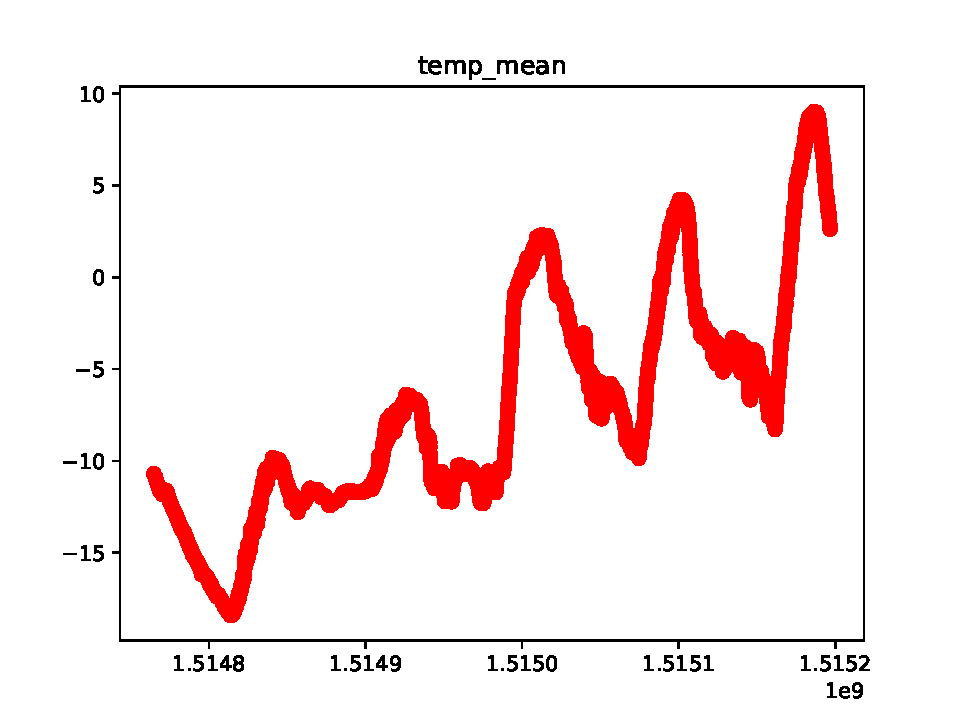
\includegraphics[width=0.6\textwidth]{../plots/temp_mean.pdf}
    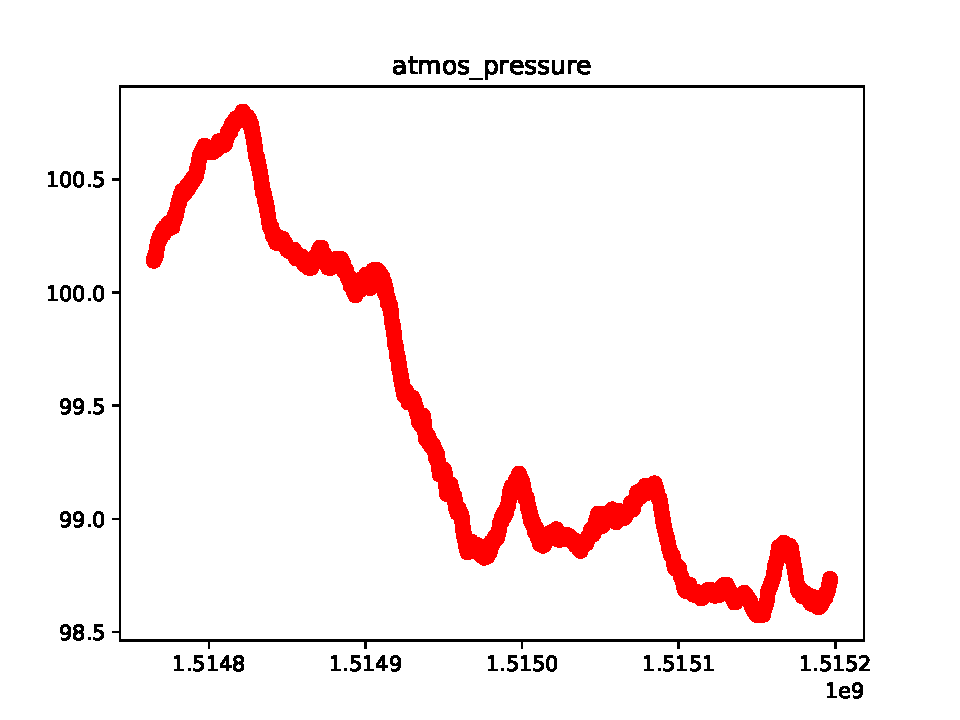
\includegraphics[width=0.6\textwidth]{../plots/atmos_pressure.pdf}
    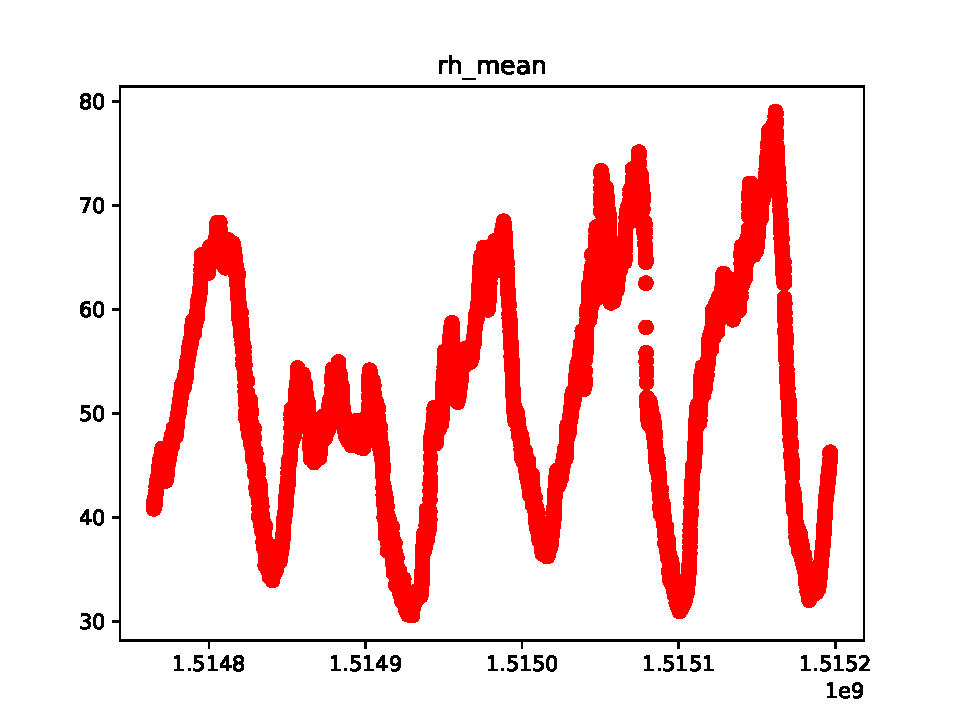
\includegraphics[width=0.6\textwidth]{../plots/rh_mean.pdf}
    \caption{Time series of the mean temperature, mean relative humidity and atmospheric pressure as a function of time.}
\end{figure}
\begin{figure}
    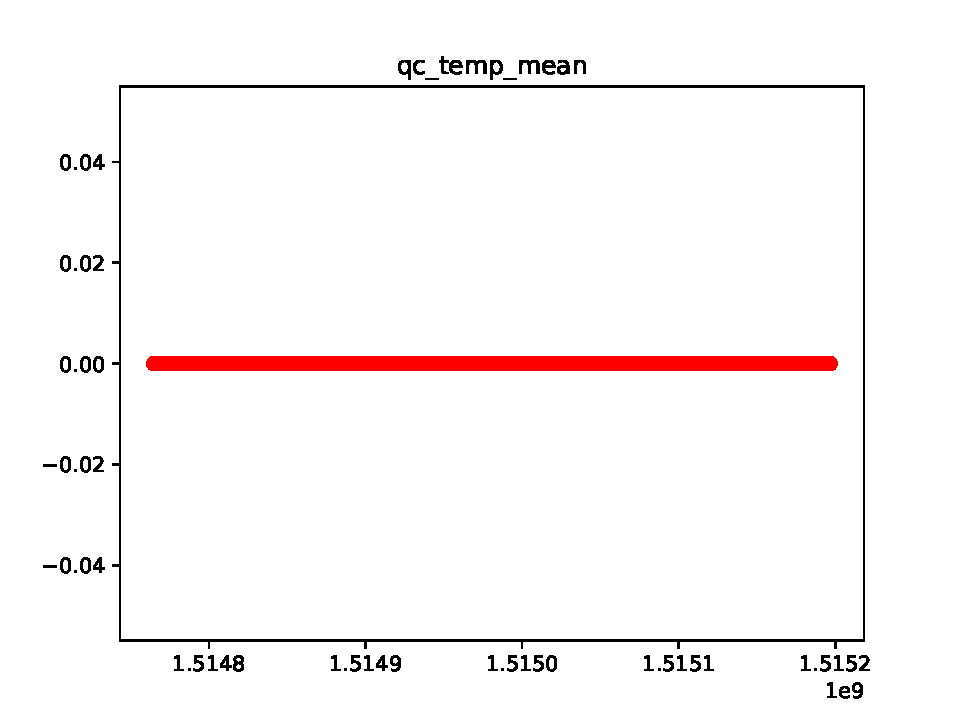
\includegraphics[width=0.6\textwidth]{../plots/qc_temp_mean.pdf}
    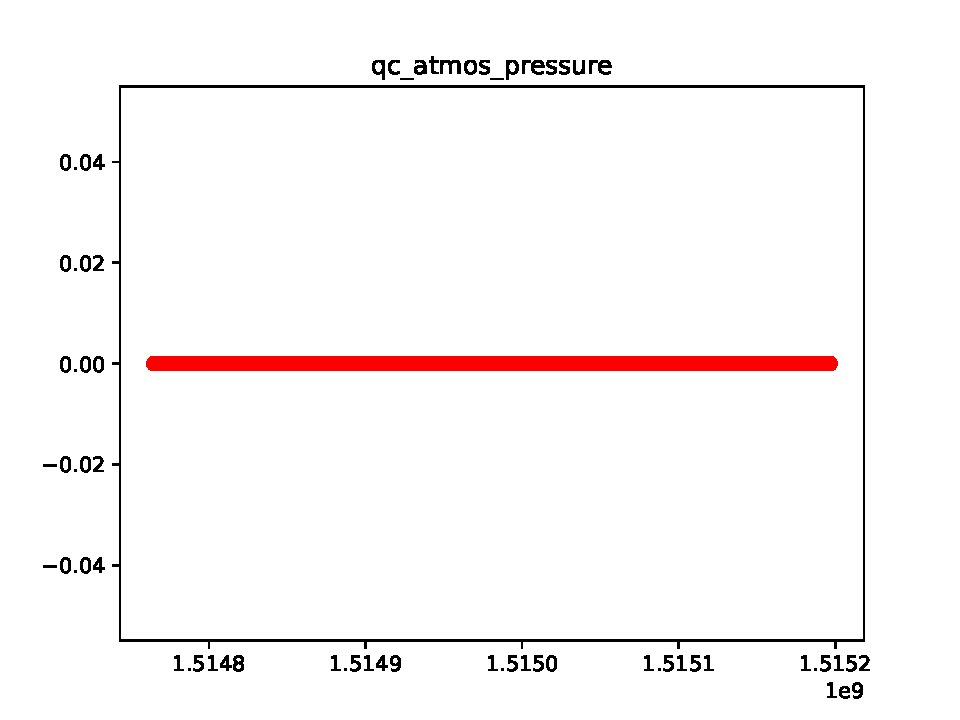
\includegraphics[width=0.6\textwidth]{../plots/qc_atmos_pressure.pdf}
    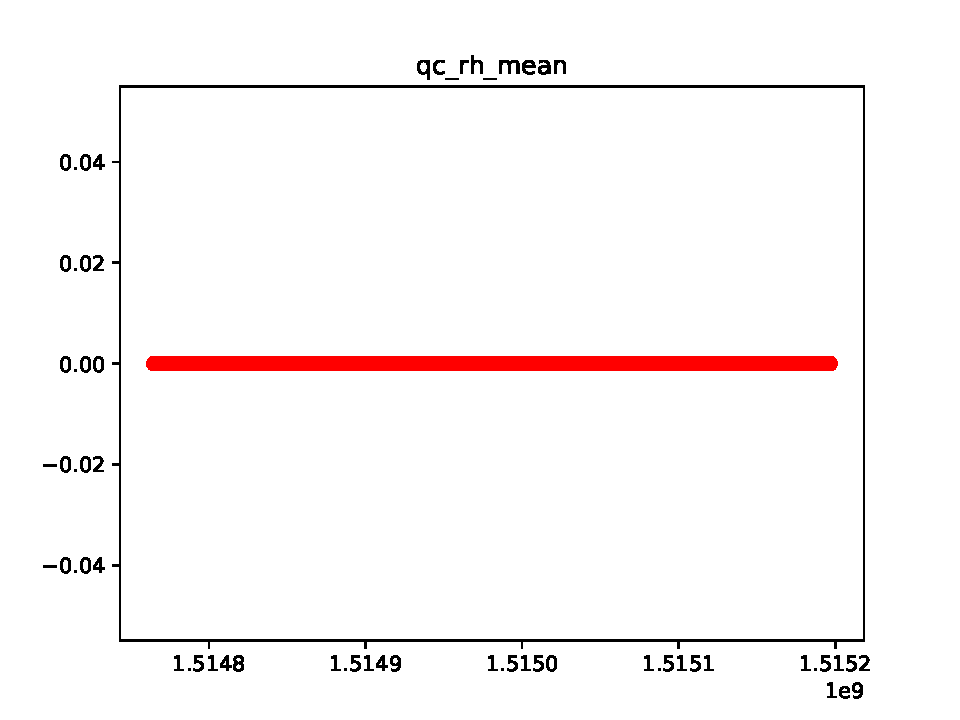
\includegraphics[width=0.6\textwidth]{../plots/qc_rh_mean.pdf}
    \caption{Time series of the quality checks for mean temperature, mean relative humidity and atmospheric pressure as a function of time.}
\end{figure}

Each file corresponds to a day of data, one data point every 60 seconds.
Each day has its own time stamp (number of seconds since midnight) and a hardcoded-modification of the reader function is required to get things working.

\subsection{Estimating the optimal average period}

Using an Allan representation of the data, I can estimate what the typical period where the measurements fluctuations are Gaussian is.
It seems that the value at which non Gaussian fluctuations appear is defined for all three variables to be about 60 samples.
For safety, I will use 50 samples for averaging.

\begin{figure}
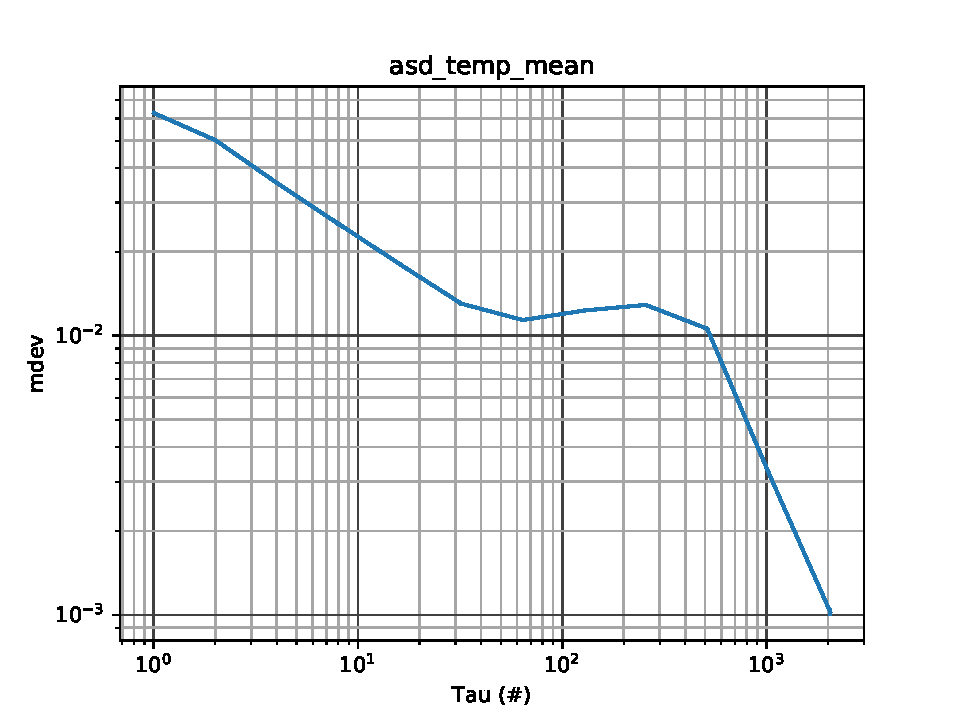
\includegraphics[width=0.6\textwidth]{../plots/asd_temp_mean.pdf}
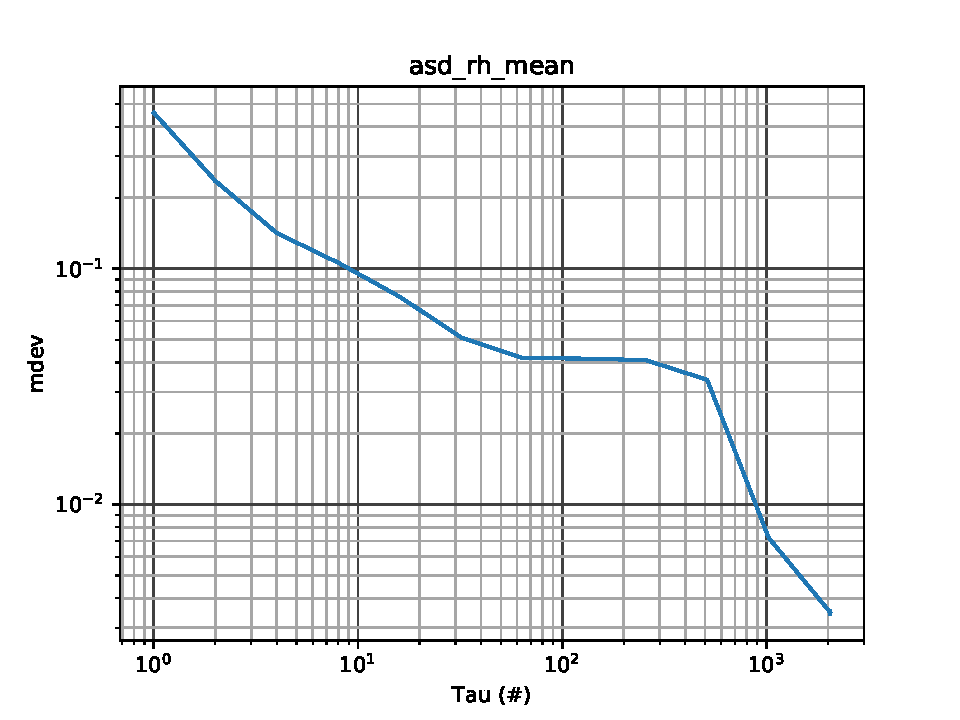
\includegraphics[width=0.6\textwidth]{../plots/asd_rh_mean.pdf}
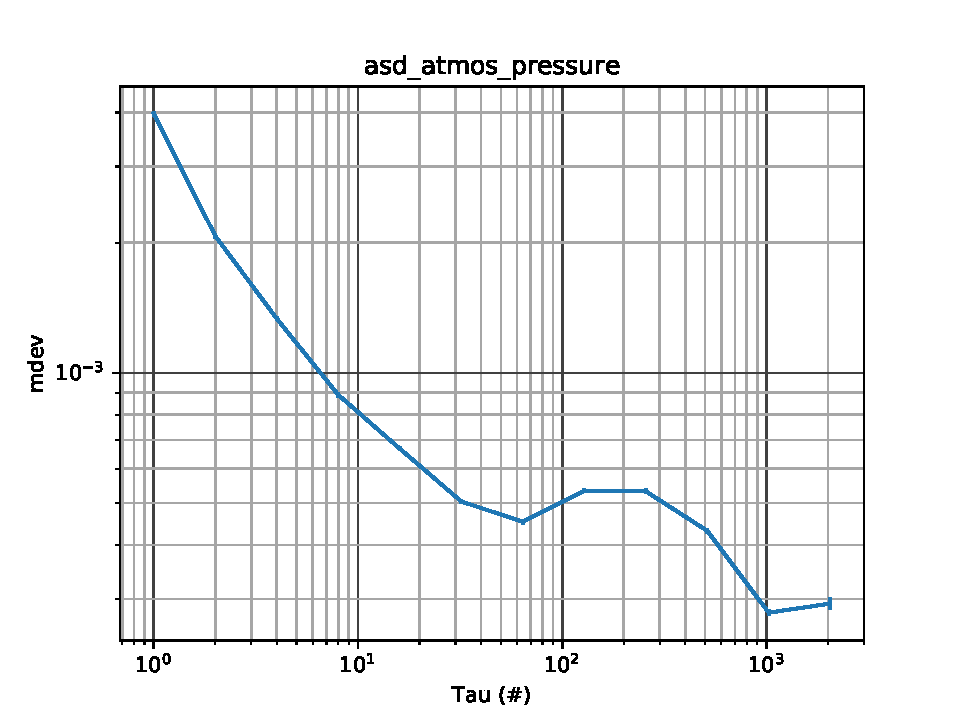
\includegraphics[width=0.6\textwidth]{../plots/asd_atmos_pressure.pdf}
\caption{Allan Standard Deviation of the mean temperature, mean relative humidity and atmospheric pressure as a function of the period (in number of samples).}
\end{figure}

{\tgf Implement an algorithmic way to extract the right number of measurements to average (something like a minimum finder).}

The averaged data (represented on Figure \ref{}) are then saved in a CDF file.
\begin{figure}
    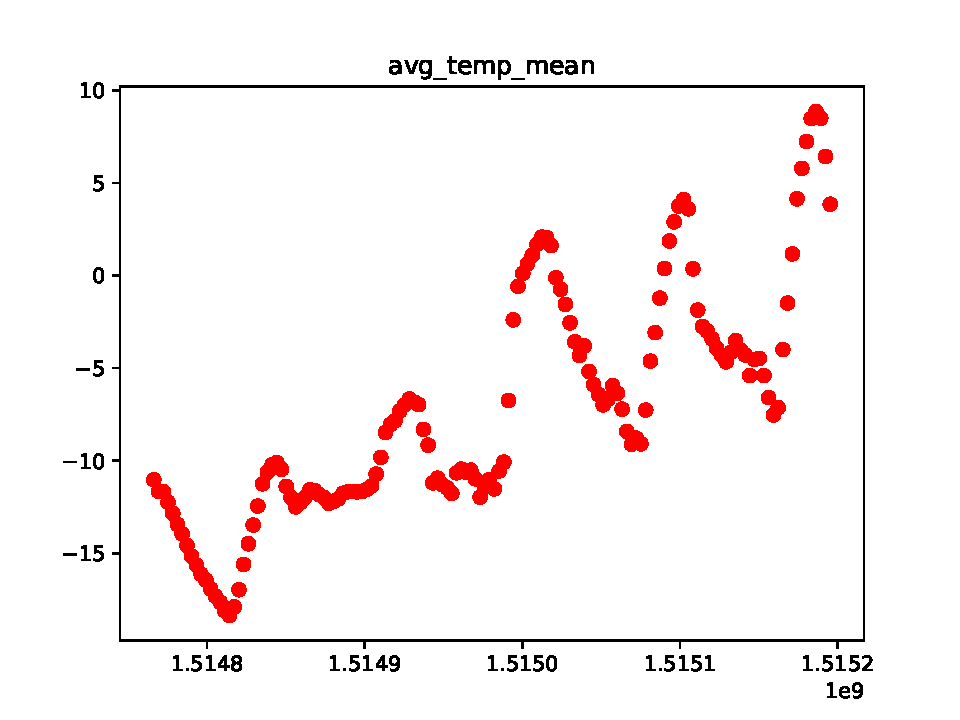
\includegraphics[width=0.6\textwidth]{../plots/avg_temp_mean.pdf}
    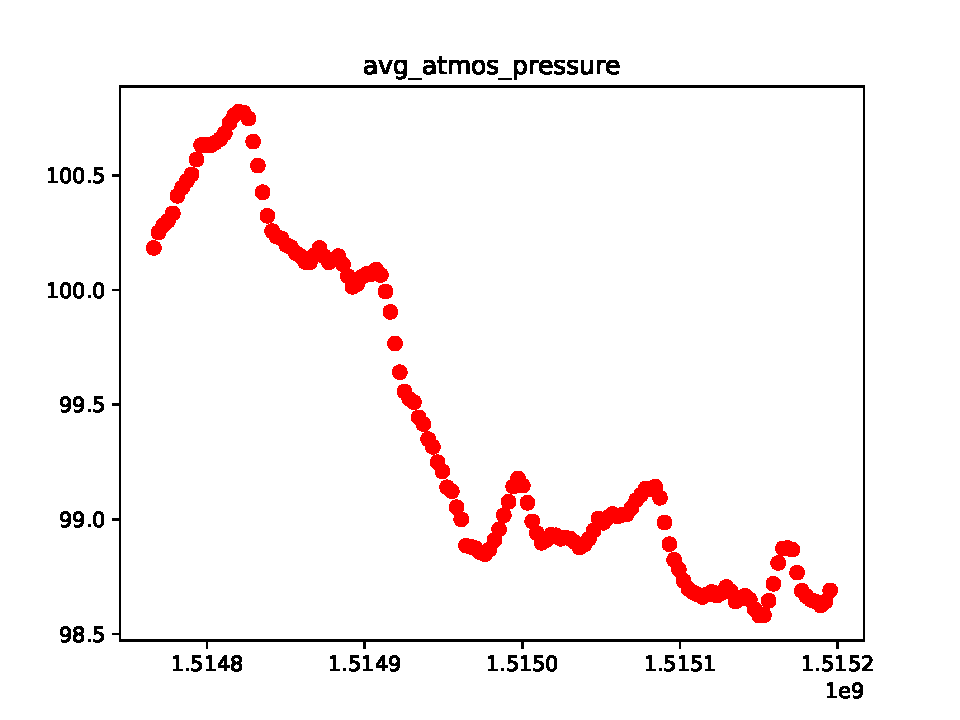
\includegraphics[width=0.6\textwidth]{../plots/avg_atmos_pressure.pdf}
    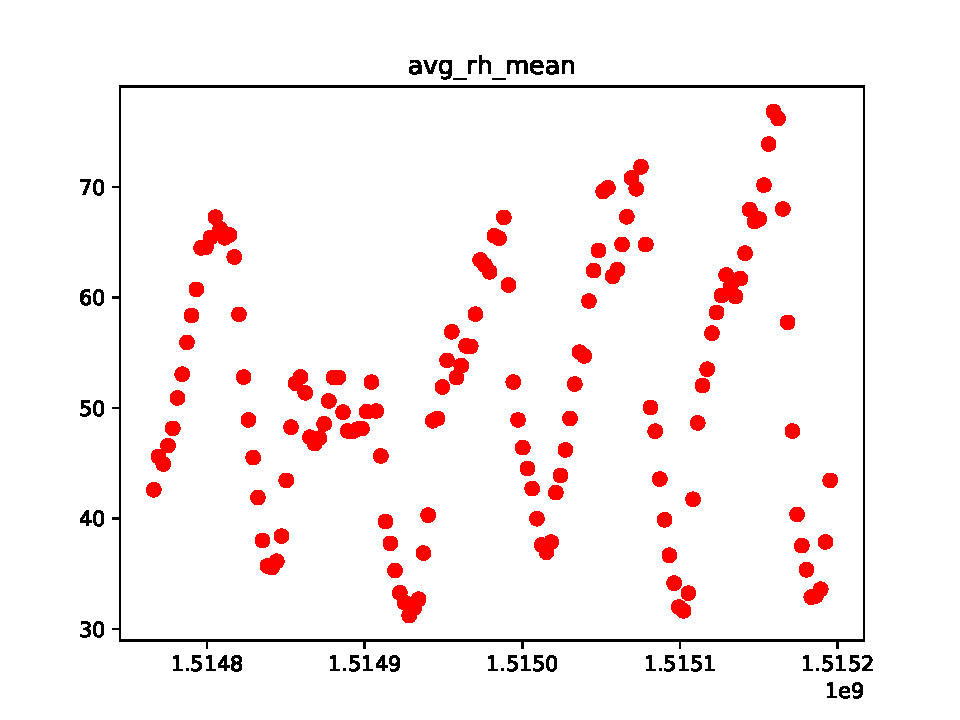
\includegraphics[width=0.6\textwidth]{../plots/avg_rh_mean.pdf}
    \caption{Time series of the average of mean temperature, mean relative humidity and atmospheric pressure as a function of time.}
\end{figure}

\section{Part 2: Clustering of data}



\end{document}  